\section{Umsetzung}
\label{sec-5}
\fbox{
\parbox{\linewidth}{
	\textit{Ziel des Kapitels:}\\
	Umsetzung erläutern: Wie wurde die Lösungsidee umgesetzt?
}}\\

Im folgenden soll erläutert werden, wie der zuvor erarbeitete Lösungsansatz umgesetzt wurde. Dazu gibt das Kapitel zunächst einen Überblick über das System und die Architektur der Anwendung. Nach einer kurzen Erläuterung zu ''Screen-Captures'' von der HoloLens folgt eine nähere Betrachtung dessen, wie die Hologramme umgesetzt wurden. Schließlich werden Details zur Interaktion und Performance genannt.

\subsection{Aufbau des Systems}
Das System ist als Client-Server-Architektur realisiert, einen Überblick gibt das Schema in Abb. \ref{img:communication-schema}. Ein Server erfasst und verarbeitet die in der Schaltung gemessenen Werte für die Stromstärke. Diese stammen von einem Arduino, der in den Stromkreislauf eingekoppelt ist. Die Applikation auf der HoloLens tritt als Client auf und erfragt die aktuellen Werte vom Server. 
\begin{figure}[H]
	\centering
	\includegraphics[width=1\textwidth]{images/todo.jpg}
	\caption{Schema Kommunikation Schaltung Arduino Server HoloLens}
	\label{img:communication-schema}
\end{figure}

\subsubsection{Client-Server Datenübertragung}
Die Übertragung der Messwerte vom Arduino zur Anwendung ist so konzipiert, dass Änderungen in Echtzeit übermittelt werden, ohne das unnötiger Netzwerktraffic entsteht. Der Client betreibt ein Polling gegen den Server, der jedoch Antworten solange zurückhält, bis ein neuer, vom vorigen abweichender Wert gemessen wurde. Dieses Verhalten veranschaulicht das Sequenzdiagramm in Abbildung \ref{img:Sequenzdiagramm}. Das Vorgehen führt dazu, dass Änderungen durch den Nutzer am Regler der Spannungsquelle ohne wahrnehmbare Verzögerung auf der HoloLens ankommen.

\vspace{8px}
\begin{center}
	\fbox{
		\parbox{0.9\linewidth}{
			\vspace{4px}
			\textbf{Überblick}
			\begin{itemize}[rightmargin=12px, topsep=-12px]
				\setlength{\itemsep}{-1pt}
				\singlespacing
				\item HoloLens erfragt Daten vom Server über HTTP GET-Requests
				\item Anfragen erfolgen asynchron
				\item Server nimmt den Request entgegen und hält eine Antwort solange zurück, bis ein neuer Wert vom Arduino vorliegt
				\item Dadurch kommen neue Daten sehr schnell bei der HoloLens an, der Nutzer sieht die Änderungen auf der Brille sofort, wenn er Änderungen an der Spannungsquelle vornimmt
				\item So wird zeitliche Einbettung und Kontinuität erreicht
				\item Dabei wird jedoch kein unnötiger Traffic erzeugt, wenn es keine Änderungen gibt
			\end{itemize}
			\vspace{18px}
	}}\\
\end{center}
%\vspace{6px}

\begin{figure}[H]
	\centering
	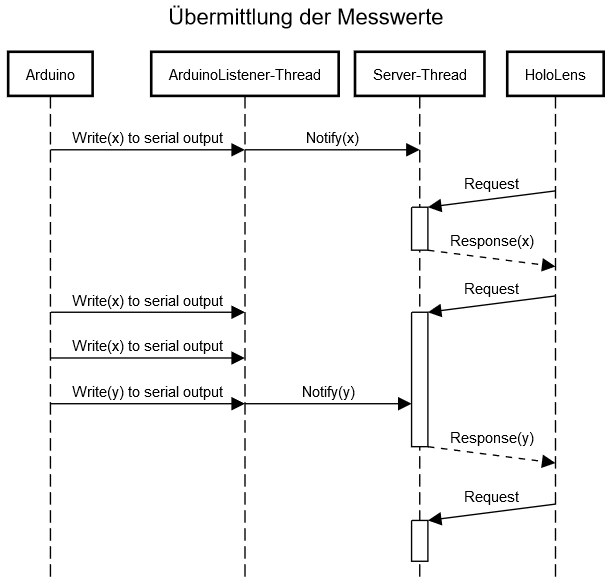
\includegraphics[width=1\textwidth]{images/Sequenzdiagramm.png}
	\caption{Sequenzdiagramm Kommunikation}
	\label{img:Sequenzdiagramm}
\end{figure}

\textit{Server}\\
Der Server besteht aus zwei miteinander kommunizierenden Threads. Ein Thread übernimmt das Lesen und Verarbeiten der Rohdaten, die über die serielle Schnittstelle eintreffen. Bei signifikanten Änderungen wird der zweite Thread mittels einer gemeinsamen, synchronisierten Variablen über die neuen Werte informiert. Dieser beantwortet daraufhin einen ggf. ausstehenden Request vom Client. Ab wann eine Änderung als signifikant gewertet wird, lässt sich über einen Threshold einstellen. Der Server wurde mit Python und der Bibliothek pyserial umgesetzt.\\

\textit{Client}\\
Der Client stellt durch die Nutzung von asynchronen Anfragen sicher, dass die Anfragen nicht blockieren. Unity bietet nur einen Thread, synchrone Anfragen würden daher zu einer Blockierung des Renderprozesses führen und so die Framerate beeinträchtigen. Da die Framerate bei 60 Hz gedeckelt ist und eine Antwort frühestens im nächsten Frame bearbeitet werden kann, beträgt die minimale Antwortzeit ca. 17 ms. Das ist ausreichend, um keine wahrnehmbare Verzögerung aufkommen zu lassen, da die Paketlaufzeit in einem lokalen Netzwerk typischerweise im einstelligen Millisekundenbereich liegt. Eine zusätzliche Wartezeit zwischen Requests kann außerdem eingestellt werden.\\

\subsubsection{Architektur der HoloLens-Anwendung}
Der Hauptteil des Systems besteht in der auf der HoloLens laufenden Applikation. Die Anwendung basiert auf der Unity Engine und wird als UWP App bereitgestellt. Das Schema in Abb. \ref{img:components-schema} gibt einen Überblick über die verschiedenen Komponenten der Anwendung. Deren Aufgaben sind in der darunter zu findenden Tabelle kurz zusammengefasst.

\begin{figure}[H]
	\centering
	\includegraphics[width=1\textwidth]{images/todo.jpg}
	\caption{Schema Komponenten}
	\label{img:components-schema}
\end{figure}


\vspace{8px}
\begin{center}
	\fbox{
		\parbox{0.9\linewidth}{
			\vspace{4px}
			\textbf{Überblick}	
\bgroup
\setlength\extrarowheight{-2pt}
\def\arraystretch{2}
\begin{table}[H]
	\centering
	\begin{tabular}{m{2.5cm}|m{8cm}}
		Komponente & Funktion\\
		\hline
		\hline
		Menu & Hauptmenü, steuert den Ablauf der Anwendung\\
		\hline
		Settings & Lädt und Speichert Einstellungen, bietet Zugang zu den Werten für andere Komponenten und steuert die Einstellungs-Oberfläche\\
		\hline
		Physics & Übernimmt alle physikalischen Berechnungen. Alle relevanten physikalischen Parameter lassen sich konfigurieren.\\
		\hline
		Tracking & Führt durch den Prozess der Positionsbestimmung und setzt den World Anchor\\
		\hline
		Model Anchor & Dient als Anker- und Container-Objekt für die einzelnen Darstellungskomponenten. Dazu gehören: Verdeckungsmodell, Kompass, die Magnetfeldmodelle, die Stromrichtungsindikatoren und das Datenpanel.\\
		\hline
		Webservice & Übernimmt die Kommunikation mit dem Server und gibt erhaltene Daten weiter\\
		\hline
		Interaction & Verarbeitet Input und Ablaufsteuerung, soweit dies nicht an einem konkreten Objekt abgewickelt wird wie z.B. Spracheingabe.\\
	\end{tabular}\caption{\label{tab:components-details} Aufgaben der einzelnen Komponenten}
\end{table}
\egroup
%\vspace{18px}
}}\\
\end{center}
\vspace{6px}

Eine Komponente besteht aus einer Hierarchie von Unity's GameObjects, die mit entsprechenden Skripten versehen sind. Die Komponenten kommunizieren auf unterschiedliche Weise miteinander. Die Behandlung von Events z.B. aufgrund von Nutzereingaben oder neuen Messwerten erfolgt über Callbacks. Manche Komponenten sind auch Singletons, auf die direkt zugegriffen werden kann wie z.B. die Einstellungen. 

\subsection{Darstellungen}
Nachdem die grundlegende Architektur der vorgestellt wurde folgt nun eine genauere Betrachtung der Umsetzung der Darstellungen. Die Ausführungen werden dabei durch Abbildungen in Form von Screenshots unterstützt. Einen ersten Eindruck vermitteln die Fotos in Abb. \ref{img:HL_SS_Intro}. Damit die von der HoloLens stammenden Bilder richtig interpretiert werden können, sind jedoch einige Vorbemerkungen nötig.

\begin{figure}[h!]
	\centering
	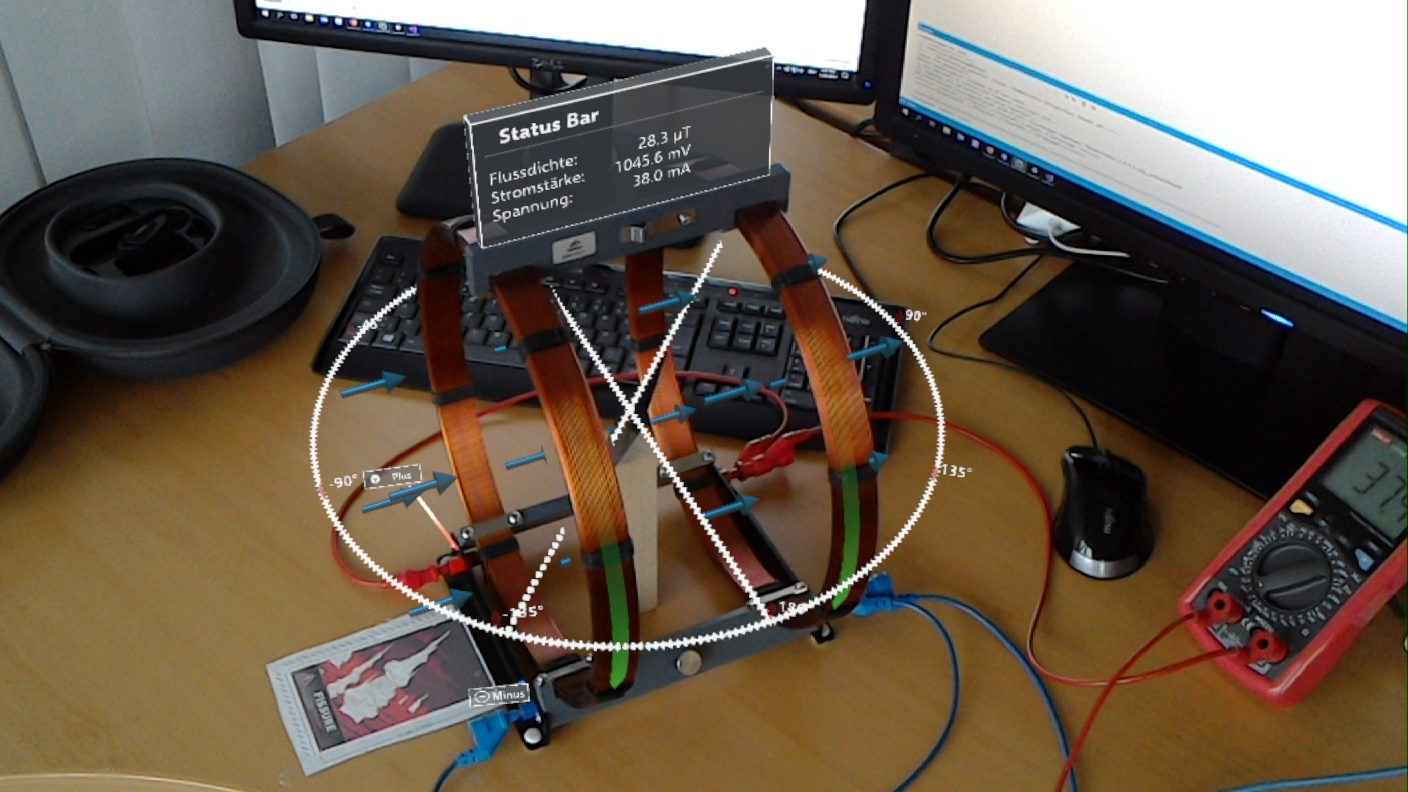
\includegraphics[width=\textwidth]{images/HL_SS1.jpg}

	\vspace{0.25cm}

	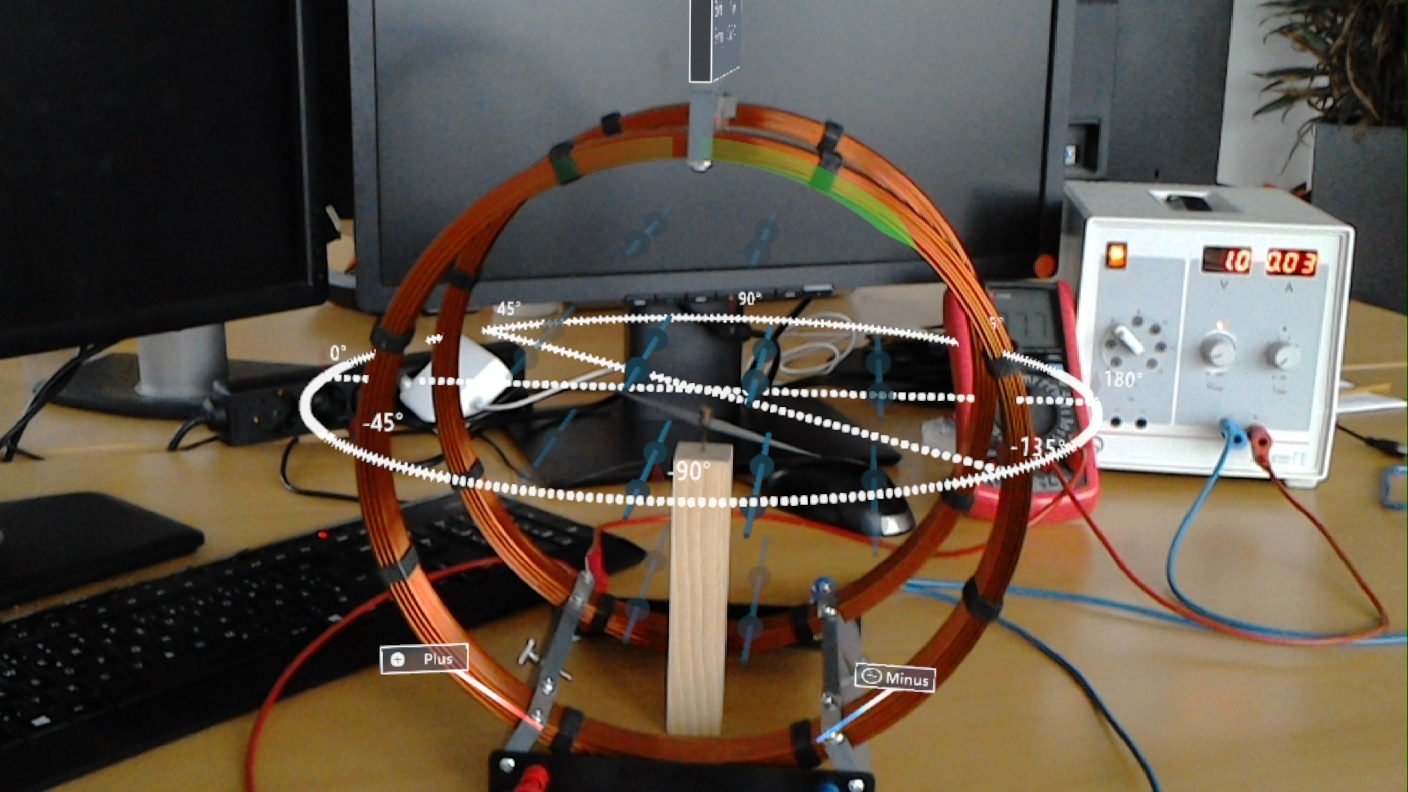
\includegraphics[width=\textwidth]{images/HL_SS2.jpg}
	\caption{Erster Eindruck HoloLens}
	\label{img:HL_SS_Intro}
\end{figure}

\subsubsection{Aufnahmen mit der HoloLens}
Zunächst ist festzuhalten, dass herkömmliche Screen-Captures auf der HoloLens nur eingeschränkt sinnvoll wären. Hier wären nämlich nur die gerenderten Objekte sichtbar, die so auch in einer Entwicklungsumgebung zu sehen sind. Die Nutzererfahrung entsteht jedoch durch das Zusammenspiel mit dem Hintergrund. Deshalb bietet die HoloLens eine angepasste Funktion, um möglichst das abzubilden, was der Nutzer tatsächlich sieht: Das \textit{Mixed Reality Capture (MRC)}.\\

Mit dem Mixed Reality Capture lassen sich Screenshots und Screen-Videos aufnehmen. Dazu nutzt die Brille ihre integrierte Frontkamera und überlagert deren Bild mit dem gerenderten Bild. So lässt sich besser darstellen, was ein Nutzer sieht. Allerdings bringt dieses Vorgehen mehrere Einschränkungen mit sich, durch die die Resultate von den tatsächlich wahrgenommenen Bildern abweichen. Damit die folgenden Bilder richtig eingeordnet werden können, sollen die wichtigsten Faktoren hier genannt werden.

\begin{itemize}
	\item Auflösung
	\item Begrenzungen des Sichtfeldes
	\item Farbe und Transparenz
	\item Positionierung
\end{itemize}

Bei einem MRC-Foto ändert sich die Auflösung von 1268x720 (720p) zu 1408x792. Obwohl die Auflösung steigt ist damit dennoch ein wesentlicher Qualitätsverlust verbunden, da der Betrachter auf der HoloLens zwei HD-Bilder sieht (stereoskopisch), beim Foto aber nur ein Bild erzeugt wird. Außerdem geht die höhere Auflösung des Einzelbildes nicht mit einer höheren Pixeldichte einher, sondern mit einem größeren Sichtfeld. Ein Foto repräsentiert daher nicht die tatsächlichen Begrenzungen des FOV. Dazu kommt die Transparenz von virtuellen Objekten. Diese hängt stark von deren Farbe sowie der Hintergrundhelligkeit ab und entspricht nicht immer der Wahrnehmung des Nutzers. Farbige Objekte erscheinen auf Fotos stets etwas transparent, auch wenn sie den Hintergrund aus Sicht des Nutzers vollständig überdecken. Das trifft z.B. auf die blauen Objekte in den Fotos aus Abb. \ref{img:HL_SS_Intro} zu. Nicht zuletzt ist auch für Fotos die Reduktion der Bildwiederholrate auf 30Hz relevant. Denn dadurch werden die Objekte nicht so gut stabilisiert und es kann zu leichten Verschiebungen auf den Fotos kommen.\\

Darüber hinaus gibt es Faktoren, die durch ein Foto nicht abgedeckt werden können. Dazu gehören die schon erläuterten Eigenheiten der stereoskopischen Wahrnehmung. Auf einem Foto sieht ein Objekt immer scharf aus und es gibt keine Probleme mit der Akkommodation oder Konvergenz, auch wenn ein Nutzer diese möglicherweise erfährt. Außerdem nimmt ein Nutzer die Umgebung anders wahr als auf einem Foto, da das Sichtfeld (auf die Umgebung) kaum eingeschränkt wird und nicht in Farbe und Auflösung begrenzt ist, sondern direkt wahrgenommen wird.\\

Diese Faktoren gilt es beim Einsatz von solchen Screen-Captures zu berücksichtigen. Prinzipiell sind auch Aufnahmen möglich, die näher an die tatsächliche Nutzererfahrung heranreichen. Diese erfordern aber weiteres Equipment, das im Rahmen dieser Arbeit nicht zur Verfügung stand.



\subsubsection{Das Magnetfeld}
Die Darstellung des Magnetfeldes in Echtzeit erfolgt über 3D-Objekte. Die Geometrie wurde mit Blender erstellt und in Unity importiert. Die Fotos in Abb. \ref{img:mfield-result} zeigen die beiden alternativen Darstellungsmodelle. Darüber hinaus steht eine Visualisierung einer vorberechneten Lösung zur Verfügung, auf die an späterer Stelle genauer eingegangen wird.

\begin{figure}[H]
	\centering
	\includegraphics[width=0.45\textwidth]{images/todo.jpg}
	\hspace{0.05cm}	
	\includegraphics[width=0.45\textwidth]{images/todo.jpg}
	\caption{Links Feldlinien Rechts Vektoren}
	\label{img:mfield-result}
\end{figure}

\vspace{4px}
\begin{center}
	\fbox{
		\parbox{0.9\linewidth}{
			\vspace{4px}
			\textit{Allgemeines}
			\begin{itemize}[rightmargin=12px, topsep=-12px]
				\setlength{\itemsep}{-1pt}
				\singlespacing
				\item Komponenten des Feldes (Erde, Spule) werden mit verschiedenen Farben dargestellt
				\item Feld der Erde ist fest und wird exemplarisch, mittig in der Spule mit der minimal notwendigen Anzahl Elemente gezeigt
				\item Feldlinien / Vektoren als Pfeillinien / Pfeile modelliert
				\item Form wird durch Schattierung betont
				\item Anordnung, Minimum und Maximum (von Abstand bzw. Länge) der Darstellungen sind im Code parametrisiert 
				\item Darstellungsgrenzen über Transparenz (Minimum) und Hardware-Limitierung (Maximum)
			\end{itemize}
			\vspace{18px}
	}}\\
\end{center}
\vspace{6px}

\textit{Visuelle Gestaltung}\\
Die Darstellung des Feldes erfolgt über 3D-Pfeile bzw. -Pfeillinien. Diese werden schattiert, damit die Form und Ausrichtung im Raum besser erkennbar wird. Beide verwenden dafür den gleichen Shader. Die Größe der Objekte wurde anhand von Erfahrungswerten angepasst. Durchmesser und Länge sind vergleichbar mit denen eines Kugelschreibers oder dickeren Stiftes. Als Farben wurden Hellblau und Orange für den Anteil der Spule bzw. der Erde gewählt. Blau wird oft für Magnetfeldlinien verwendet und wird daher auch hier gebraucht. Allerdings wird ein weniger gesättigtes, helleres Blau verwendet, damit die Deckkraft vor helleren Hintergründen nicht verloren geht. Das Orange weißt die selbe Sättigung und Helligkeit auf wie das Blau, damit sich die Objekte nicht in der Transparenz voneinander unterscheiden.\\

\textit{Begrenzung der Darstellung}\\
Die Visualisierung des Feldes erfordert die Festlegung eines darzustellenden Bereiches für die Flussdichte. Ein Intervall lässt sich in der Anwendung frei über die Einstellungen festlegen. Diese Einstellungsmöglichkeit ist für die praktische Nutzung wesentlich, da die gemessene Flussdichte des Erdmagnetfeldes in Abhängigkeit von der Umgebung variieren kann. Voreingestellt ist ein Bereich von $3\mu T$ bis $60\mu T$, die Flussdichte der Erde liegt mit $30 \mu T$ bis $40 \mu T$ im mittleren Bereich dieser Skala. Am unteren Ende des Bereiches werden die Objekte über Transparenz ausgeblendet.\\

Nach oben hin ist keine Darstellung der Begrenzung vorgesehen. Der Bereich sollte so gewählt werden, dass die obere Grenze durch die maximal am Regler einstellbare Stromstärke nicht erreicht werden kann. Somit erfährt der Anwender die Limitierung der Darstellung auf natürliche Weise. Die Konfiguration der Schaltung kann hier über eingebaute Widerstände so an die Spannungsquelle angepasst werden, dass der erzeugte Stromfluss im gewünschten Bereich liegt.\\

\textbf{Feldlinien}\\
Die Feldliniendarstellung ist in Abb. \ref{img:mfield-lines} gesondert abgebildet.
\begin{figure}[H]
	\centering
	\includegraphics[width=0.45\textwidth]{images/todo.jpg}
	\caption{Feldlinien}
	\label{img:mfield-lines}
\end{figure}
\vspace{4px}
\begin{center}
	\fbox{
		\parbox{0.9\linewidth}{
			\vspace{4px}
			\textit{Überblick}
			\begin{itemize}[rightmargin=12px, topsep=-12px]
				\setlength{\itemsep}{-1pt}
				\singlespacing
				\item Pfeillinien repräsentieren Feldlinien über Abstand und Ausrichtung
				\item 4 bis 16 Feldlinien im Gitter angeordnet, orthogonal zur Z-Achse
				\item Anordnung im 3D-Gitter mit konfigurierbaren Parametern (Abstand, Anzahl pro Dimension)
				\item Änderung des Abstandes über Kontraktion zum Mittelpunkt in X-Y-Ebene, Linien werden über Transparenz an der Darstellungsgrenze ein- bzw. ausgeblendet
			\end{itemize}
			\vspace{18px}
	}}\\
\end{center}
\vspace{6px}
\textit{Anordnung}\\
Die Feldlinien der Spule verlaufen orthogonal zur X-Y-Ebene, also in Richtung der Z-Achse. Damit die gewünschten Eigenschaften (Stärke, Homogenität und Richtung) des dreidimensionalen Feldes anhand des Feldlinienmodells erkennbar sind, bedarf es mindestens vier Linien. In einer 2x2 Anordnung um den Mittelpunkt der X-Y-Ebene ist so der Abstand in beiden Dimensionen sichtbar und die Linien sind symmetrisch zur Z-Achse. Anhand der Parallelität lässt sich die Homogenität erkennen und anhand des Abstandes (in der horizontalen oder vertikalen, beide sind gleich groß) die Stärke. Die Flussrichtung ist über eingebaute Pfeilspitzen abgebildet. Als Darstellungsvolumen wurde ein zylindrischer Ausschnitt der Spule gewählt, da diese den Raum besser ausfüllt, als beispielsweise ein kubischer Ausschnitt.\\

\textit{Anzahl}\\
Bei einem festen, für die Darstellungen zur Verfügung stehenden Volumen und kleiner werdenden Abständen müssen zunehmend mehr Linien gezeichnet werden. Zu viele Objekte würden jedoch die Sichtbarkeit anderer Elemente wie Magnetnadel und Kompass beeinträchtigen. Außerdem transportieren zusätzliche Feldlinien keine zusätzlichen Informationen (im Fall eines homogenen Feldes). Allerdings unterstützt die Beobachtung, dass mit zunehmender Flussdichte die Anzahl der Feldlinien steigt, das Verständnis des Feldlinienmodells. Daher wurde für die Umsetzung das Intervall von minimalem und maximalem Abstand so gewählt, dass mindestens 4 und höchstens 16 Linien dargestellt werden. Beim Ein- und Austreten der Objekte in das bzw. aus dem Darstellungsvolumen werden sie kontinuierlich ein bzw. ausgeblendet.\\

\begin{figure}[H]
	\centering
	\includegraphics[width=0.45\textwidth]{images/todo.jpg}
	\caption{Feldlinien Skalierung Abstand}
	\label{img:mfield-lines-scaling}
\end{figure}

\textit{Skalierung}\\
Dabei wurde sich bewusst für die Abbildung der Flussdichte auf den Abstand der Feldlinien entschieden. Das bedeutet, Letzterer ändert sich proportional mit der Flussdichte. Oft wird statt des Abstandes die Anzahl der Feldlinien durch eine Einheitsfläche proportional zur Flussdichte gewählt. Das bedeutet bei einer symmetrischen Darstellung eines quadratischen Ausschnittes jedoch, dass die Anzahl in diskreten Stufen $n \geq 1$ mit $4^{n}$ steigt. Werden diese Stufen durch eine kontinuierliche Kontraktion der Linien zum Zentrum hin interpoliert, dann skaliert der Abstand $d$ der Feldlinien mit $1/(3n)$. Die Grafik \ref{img:mfield-lines-scaling} illustriert diesen Zusammenhang. Da für den Anwender in erster Linie jedoch der Abstand die sichtbare, sich ändernde Größe ist, könnte dies den falschen Eindruck erwecken, die Flussdichte ändere sich nicht linear mit der Stromstärke. Außerdem werden nur zwei Stufen dargestellt, daher wurde sich für die proportionale Änderung des Abstandes entschieden.\\

\textbf{Vektoren}\\
Die Umsetzung der Vektordarstellung ist in Abb. \ref{img:mfield-vectors} näher zu sehen.
\begin{figure}[H]
	\centering
	\includegraphics[width=0.45\textwidth]{images/todo.jpg}
	\caption{Vektoren}
	\label{img:mfield-vectors}
\end{figure}
\vspace{4px}
\begin{center}
	\fbox{
		\parbox{0.9\linewidth}{
			\vspace{4px}
			\textit{Überblick}
			\begin{itemize}[rightmargin=12px, topsep=-12px]
				\setlength{\itemsep}{-1pt}
				\singlespacing
				\item Pfeile repräsentieren Flussdichtevektor über Länge und Ausrichtung
				\item 8 Pfeile für homogenes Feld, weitere 8 für Andeutung inhomogenes Feld
				\item Anordnung im 3D-Gitter mit konfigurierbaren Parametern (Abstand und Anzahl, jeweils pro Raumrichtung)
				\item Ankerpunkt mittig im Pfeil
			\end{itemize}
			\vspace{18px}
	}}\\
\end{center}
\vspace{6px}

\textit{Anordnung und Anzahl}\\
In der Vektordarstellung werden mindestens acht Vektoren benötigt, damit die zuvor genannten Eigenschaften erkennbar werden. Dabei gelten die gleichen Gründe wie zuvor. Während jedoch eine Feldlinie das Feld in Richtung der Z-Achse kontinuierlich darstellt, sind hier wenigstens zwei Vektoren notwendig. Die Anordnung erfolgt in einem 3D-Gitter, bei dem die Anzahl und die Abstände pro Dimension parametrisiert sind. Auch hier gilt, dass mehr Objekte im homogenen Teil des Feldes keine weiteren Informationen transportieren. Daher wurde in Anbetracht des zur Verfügung stehenden Raumes in die Größe anstelle der Anzahl der Objekte investiert.\\

\textit{Skalierung}\\
Die Flussdichte wird im Fall der Pfeile über deren Länge und Richtung ausgedrückt. Die Form der Objekte soll mit einer sich ändernden Länge nicht verzerrt werden. Eine einfache Skalierung der Pfeillänge würde jedoch dazu führen, dass auch die Pfeilspitze in die Länge gezogen wird. Daher wird die Geometrie zur Laufzeit angepasst und nur ein Teil in der Mitte verändert.\\

\textit{Bezugspunkt}\\
Welcher Punkt dem Vektor als Ankerpunkt dient ist dabei nicht entscheidend, denn ein Pfeil repräsentiert jeden Punkt des homogenen Feldes. Eine explizite Darstellung ist daher nicht erforderlich. Allerdings wird die Verankerung im Mittelpunkt dadurch deutlich, dass die Position bei variierender Länge gleich bleibt.\\

\textit{Inhomogener Anteil}\\
Im Gegensatz zu den Feldlinien ist eine Darstellung des inhomogenen Feldes über Vektoren auch ohne aufwendige Echtzeit-Berechnungen möglich (siehe Kap. \ref{sec-2-2-1}). Die Anwendung nutzt diese Eigenschaft, um in dieser Darstellung auch das inhomogene Feld anzudeuten. Dies geschieht, indem das Raster so gewählt wird, dass vor und hinter der Spule (im Sinne der Z-Achse) jeweils eine Reihe Vektoren positioniert ist. Diese sind hier im Vergleich deutlich kürzer und nicht parallel, sondern nach innen bzw. nach außen gerichtet. So wird erkennbar, dass das Feld hier schwächer und inhomogen ist. Da die Darstellungen erst ab einem minimalen Wert eingeblendet werden, wird der inhomogene Teil nach dem homogenen Teil eingeblendet.\\

 
\textbf{Simulation}\\
Eine Visualisierung der Simulationsdaten ist in Abb. \ref{img:mfield-simulation} näher zu sehen.
\begin{figure}[H]
	\centering
	\includegraphics[width=0.45\textwidth]{images/todo.jpg}
	\caption{Simulation}
	\label{img:mfield-simulation}
\end{figure}
\vspace{4px}
\begin{center}
	\fbox{
		\parbox{0.9\linewidth}{
			\vspace{4px}
			\textit{Überblick}
			\begin{itemize}[rightmargin=12px, topsep=-12px]
				\setlength{\itemsep}{-1pt}
				\singlespacing
				\item Feldlinien vorberechnet mit COMSOL Multiphysics, exportiert als CSV, Import in Unity erfolgt zur Laufzeit
				\item Simulation für einen beliebigen 2D-Querschnitt orthogonal zur X-Y-Ebene, da das Feld symmetrisch zur Z-Achse ist
				\item Anzahl auf 10 Feldlinien festgelegt
				\item Darstellung über 2D-Linien
				\item Rot-Grün Farbskala genutzt
			\end{itemize}
			\vspace{18px}
	}}\\
\end{center}
\vspace{6px}

Die numerische Lösung der Feldgleichungen erfolgte mittels der Simulationssoftware COMSOL Multiphysics. Diese Arbeit konnte hier auf eine bestehende Implementierung einer Helmholtzspule aufbauen. Hier wurden lediglich die folgenden Parameter für die Berechnung der Feldlinien gesetzt:
\begin{itemize}
	\item Anzahl und Anordnung: 10, symmetrisch zur Z-Achse, Abstand entsprechend der Flussdichte
	\item Beschränkung auf die X-Z-Ebene
	\item Integrationsgenauigkeit?
\end{itemize}
\textit{Export, Import, Datenformat}\\
Das Ergebnis der Simulation ist eine Liste von Datenpunkten der Form \textbf{[}\textit{FeldlinienNr:} Int, \textit{Position:} Vector3, \textit{Betrag der Flussdichte:} float\textbf{]}. Dafür wurde ein CSV-Reader geschrieben, der die Daten zur Laufzeit der Applikation einliest, interpretiert und zum Rendering an GameObjects weitergibt. Folglich ließen sich mehrere Simulationen vorberechnen und anzeigen.\\

\textit{Querschnitt}\\
Zunächst ist nur eine Anordnung in der X-Z-Ebene aktiv. Da das Feld aber symmetrisch zur Z-Achse ist, kann mit diesem einen Datensatz bereits jeder Querschnitt durch die Z-Achse dargestellt werden. Bei einer anderen Ausrichtung, z.B. im 45° Winkel, würden jedoch Feldlinien durch den Tisch verlaufen, auf dem die Spule steht.\\

\textit{Rendering}\\
Die Darstellung erfolgt über Unity's Low-Level \textit{Graphics Library (GL)} mittels eines Line-Strips. Dieser ist vergleichbar mit dem von OpenGL, hat aber weniger Funktionen. Insbesondere lässt sich die Dicke der Linien nicht einstellen, sondern ist auf einen Pixel festgelegt. Der sonst in dieser Arbeit für Linien genutzte LineRenderer konnte hier nicht verwendet werden. Denn letzterer ermöglicht für eine Linie nur die Interpolation zwischen maximal 8 Farben. Eine besser Konfigurierbare Darstellung wäre über ein dynamisch generiertes Mesh möglich.\\

\textit{Anzahl und Anordnung}\\
Die Auswahl von 10 Feldlinien erfolgte aus praktischem Ermessen bezüglich der Sichtbarkeit aus 1,5 Metern Entfernung. Dabei wurde bewusst eine gerade Anzahl gewählt. Andernfalls entsteht eine Feldlinie, die genau auf der Z-Achse liegt und nicht geschlossen ist sondern von minus nach plus Unendlich verläuft. Dies wurde aus didaktischen Gründen vermieden.\\

\textit{Farbe}\\
Die Wahl der Farbskala fiel aus mehreren Gründen auf eine Rot-Grün-Skala. Die Linien zeigen die kontinuierliche Änderung der Flussdichte, die durch einen Farbverlauf weiter hervorgehoben werden soll. Dabei kommt es nicht auf das Ablesen der numerischen Werte an, weshalb auch keine Skala mit Farbe und den dazugehörigen Werten angezeigt wird. Es geht viel mehr um das qualitative Verständnis der Darstellung. Mit der gewählten Skala unterscheiden sich die drei wesentlichen Regionen durch ihre Farbe klar voneinander:
\begin{itemize}
	\item Inhomogenes, schwaches Feld außen: Grün
	\item Homogenes, mittel-starkes Feld innen: Gelb
	\item Inhomogenes, starkes Feld unmittelbar am Rand der Spule: Rot
\end{itemize}

Darüber hinaus sprechen technische Gründe für eine solche Farbskala. Damit die Linien in Helligkeit und Transparenz nicht variieren, sollten sich die Farbanteile im RGB-Raum stets zu einem konstanten Wert addieren. Die Rot-Grün-Skala erfüllt diese Eigenschaft, da hier der Blauanteil stets null ist und Rot und Grün über $R = 1 - G$ zusammenhängen. Möglich wären hier auch eine Regenbogenskala, die jedoch aus Gründen der Wahrnehmung nicht empfohlen wird.\\

\subsubsection{Stromfluss, Kompass und weitere Darstellungen}
\textbf{Strom-Pfeile}
\begin{itemize}
	\item Darstellungen über breite 2D-Linien mit Unity's LineRenderer, die an einem Ende zu einer Pfeilspitze zusammenlaufen
	\item Liegen direkt auf der Spule auf und sind fest, richten sich also nicht zur Kamera aus
	\item Es werden stets nur Pfeile an der Seite der Spule angezeigt, die der Nutzer gerade sehen kann
	\item Dazwischen werden die Pfeile kontinuierlich ein- bzw. ausgeblendet
\end{itemize}

\textbf{Strom-Labels}
\begin{itemize}
	\item Plus- und Minus-Kennzeichner über Tooltip-Elemente des MRTK umgesetzt
	\item Verbindungslinien farblich an die Farbe der Verbindungsstücke angepasst
	\item Tooltips um Plus- und Minus-Icons ergänzt
\end{itemize}


\textbf{Kompass-Linien}
\begin{itemize}
	\item Darstellungen über gestrichelte 2D-Linien mit Unity's LineRenderer
	\item Gestrichelte Linie durch Textur mit weißem Kreis und transparentem Hintergrund, Skalierung auf die Länge der Linie mit Tiling
	\item Billboard-Verhalten für Sichtbarkeit aus unterschiedlichen Winkeln
	\item Grau als Farbe genutzt, leicht transparent, virtueller Kompass jedoch etwas heller und daher präsenter gestaltet
\end{itemize}


\textbf{Textboxen}
\begin{itemize}
	\item 4 Replikas, Platzierung an unteren Balken zwischen den beiden Spulen
	\item Sichtbarkeit analog zu Strom-Pfeilen
	\item Dunkelgrauer Hintergrund für bessere Lesbarkeit
	\item Listet gemessene und berechnete Echtzeitwerte auf: Stromstärke, Spannung, Flussdichte
\end{itemize}

\subsubsection{Weitere technische Komponenten}

\vspace{8px}
\begin{center}
	\fbox{
		\parbox{0.9\linewidth}{
			\vspace{4px}
			\textbf{Überblick}
			\begin{itemize}[rightmargin=12px, topsep=-12px]
				\setlength{\itemsep}{-1pt}
				\singlespacing
				\item Spule maßstabsgetreu für Verdeckungsberechnung modelliert mit ca. 2mm größerer Ausdehnung, Rendering ausschließlich in den Z-Puffer
				\item Near Plane Fading verbirgt Objekte, die eine minimale Distanz zur Kamera unterschreiten
				\item Progress Indikator informiert über Zustand länger laufende Vorgänge, z.B. Ladevorgang der Simulationsdaten oder Einlesen des Markers
				\item Tracking mit Vuforia, nur zum Erkennen des Markers aktiv
			\end{itemize}
			\vspace{18px}
	}}\\
\end{center}
\vspace{6px}

\textit{Occlusion Berechnung}\\
Nachmodelliert besser als Mesh, denn Mesh zu ungenau, Rendering nur in z puffer verbessert Performance, folgt Hinweis der Doku, near plane clipping beachten \\
\begin{figure}[H]
	\centering
	\includegraphics[width=0.45\textwidth]{images/todo.jpg}
	\hspace{0.05cm}	
	\includegraphics[width=0.45\textwidth]{images/todo.jpg}
	\caption{HoloLens Mesh vs. Modell}
	\label{img:mesh-vs-model}
\end{figure}

\begin{comment}
\begin{itemize}
\item Für Verdeckung werden maßstabsgetreu nachmodellierte, virtuelle Objekte verwendet
\item 3D Mesh in Blender erstellt, 2mm größer als echte Objekte für Spielraum
\item Objekte werden möglichst genau über reale gelegt
\item Rendering erfolgt ausschließlich in den Z-Puffer, dadurch sind die realen Objekte sichtbar, die virtuellen verdecken jedoch dahinterliegende, vrituelle Objekte
\item Das Near Clipping Plane muss dafür jedoch sehr nah am Kameraursprung liegen, andernfalls würden weiter entfernte, virtuelle Objekte plötzlich doch vor realen Objekten angezeigt werden, sobald letztere zu nah sind und das Clipping die Objekte vom Rendering ausschließt
\end{itemize}
\end{comment}

\textit{Near Plane Fading}\\
Minimale Distanz, angenehmer als Clipping, fade to transparent nicht umgesetzt\\
\begin{comment}
\begin{itemize}
\item Minnimum Distanz
\item Behinderung bei Interaktion mit Versuchsaufbau
\item Bessere UX als Clipping
\item MRTK Standard Shader implementiert Fade To Black
\item Lineares Fading überall genutzt
\end{itemize}
\end{comment}

\textit{Progress Indikator}\\
Bekannter Windows Ladeindikator, bereitgestellt durch MRTK\\

\textit{Tracking}\\
Vuforia Tracking Framework genutzt, eigene Sequenz führt den Nutzer durch den Prozess\\

\textit{Künstliche Beleuchtung}\\
Beleuchtung bildet grob erwartete Lichtverhältnisse nach, keine Schatten\\
\begin{comment}
\begin{itemize}
\item Virtuelle Beleuchtung von Oben bildet echte Lichtverhältnisse grob nach
\item Unterstützt die Einbettung der 3D Objekte im Raum
\end{itemize}
\end{comment}

\subsection{Interaktion}
\textbf{Erkennung der Position über eigene Sequenz in Zusammenarbeit mit dem Nutzer}
\begin{itemize}
	\item Nutzer versteht die Funktionsweise der Anwendung
	\item Nutzer erhält Feedback über den Prozess der Positionsbestimmung von der Anwendung
	\item Nutzer kann sein Verhalten anpassen und so den Prozess unterstützen
	\item Bessere Kalibrierung möglich
	\item Tracking nur für kurze Zeit erforderlich, das spart viel Ressourcen
	\item Marker verdeckt kein Teil des Sichtfeldes, kann nach Positionierung auch entfernt werden
\end{itemize}

\subsection{Performance}
Vorgenommene Optimierungen:
\begin{itemize}
	\item Single Pass Instanced rendering
	\item 16 bit depth buffer (min available)
	\item Vuforia nur für den Vorgang der Positionsbestimmung aktiv
	\item Physics Enginge deaktiviert
	\item Frustum Culling
	\item Occlusion Mesh wird auschließlich in Z-Puffer gerendert
	\item Texture MipMaps
\end{itemize}
